\documentclass[a4paper]{article}
% Esto es para que el LaTeX sepa que el texto está en español:
\usepackage[spanish]{babel}
\selectlanguage{spanish}
% Esto es para poder escribir acentos directamente:
\usepackage[utf8]{inputenc}
\usepackage[T1]{fontenc}
\usepackage{float}



%% Asigna un tamaño a la hoja y los márgenes
\usepackage[a4paper,top=3cm,bottom=2cm,left=3cm,right=3cm,marginparwidth=1.75cm]{geometry}

%% Paquetes de la AMS
\usepackage{amsmath, amsthm, amsfonts}
%% Para añadir archivos con extensión pdf, jpg, png or tif
\usepackage{graphicx}
\usepackage[colorinlistoftodos]{todonotes}
\usepackage[colorlinks=true, allcolors=blue]{hyperref}

%% Primero escribimos el título
\title{MPLS}
\author{Comunicaciones Digitales\\
  \small Isaias Gatica\\
  \small isaiasgatica1@gmail.com\\
  \date{}
}

%% Después del "preámbulo", podemos empezar el documento                    
\begin{document}
\maketitle

\begin{itemize}
    \item Problemas de red IP
    \item Se requeria mayor QoS y ancho de banda. Llega ATM
    \item Problema: Dificultad de operar e integrar una red basandose en dos tecnologias distintas.
\end{itemize}
\section{Concepto de MPLS}
MPLS es un estandar IP de conmutación de paquetes del IETF. Con IP sin conexión tradicional, la dirección
de destino junto a otros parámetros de la cabecera, es examinada cada vez que el paquete atravisa un router. La ruta
del paquete se adapta en función de las tablas de encaminamiento de cada nodo. Esto genera perdidas de tiempo y no garantiza una buena Qos.
Sin embargo, MPLS permite a cada nodo asignar una etiqueta a cada uno de los elementos de la tabla y comunicarla 
con sus nodos vecinos. Esta etiqueta es un valor corto y de tamaño fijo transportado en la cabecera del paquete para 
identificar un FEC (Forward Equivalence Class), que es un conjunto de paquetes que son reenviados
sobre el mismo camino a traves de la red. Para formar un FEC los paquetes deben:
\begin{itemize}
    \item El salto siguiente es el mismo.
    \item La misma interfaz de salida.
    \item Las mismas políticas de cola.
\end{itemize}
Si bien el concepto de FEC tambien esta presente en las comunicaciones IP normales, al usar MPLS el FEC se determina una única vez y no entre cada 
salto entre los enrutadores de la ruta de envio. \\
Por otro lado, para comprender en mas profundidad una red MPLS es necesario conocer los siguientes conceptos:
\begin{itemize}
    \item LSP (\textit{Label Switch Path}): establece un camino a traves de la RED y se reservan los recursos físicos 
    necesarios para satisfacer los requerimientos previamente definidos. Se crea utilizando protocolos específicos.
    \item Partes de la red:
    \begin{itemize}
        \item LER (\textit{Label Edge Routers}): router o switch el cual analiza la dirección de IP de destino y la QoS para definir la 
        etiqueta MPLS que identifica en que LSP se encuentra el paquete. De esta forma establece (a traves de la etiqueta) el camino entero que debe seguir el paquete 
        a lo largo de la red.
        \item LSR (\textit{Label Switching Routers}):router o switch el cuál esta ubicado en el núcleo de la red. Son los encargados de encaminar los 
        paquetes por la red. Cuando llega un paquete, lee el valor de la etiqueta de entrada de la cabecera MPLS y busca en la tabla de conmutación la nueva etiqueta MPLS y la interfaz de salida. Hecho esto reenvia el 
        paquete por el camino predefinido (LSP) con la nueva etiqueta, si el próximo salto es hacia un LER no es necesaria etiqueta entonces extrae la cabecera MPLS reduciendo cabeceras innecesarias.
    \end{itemize}
\end{itemize}
\begin{figure}[H]
    \centering
    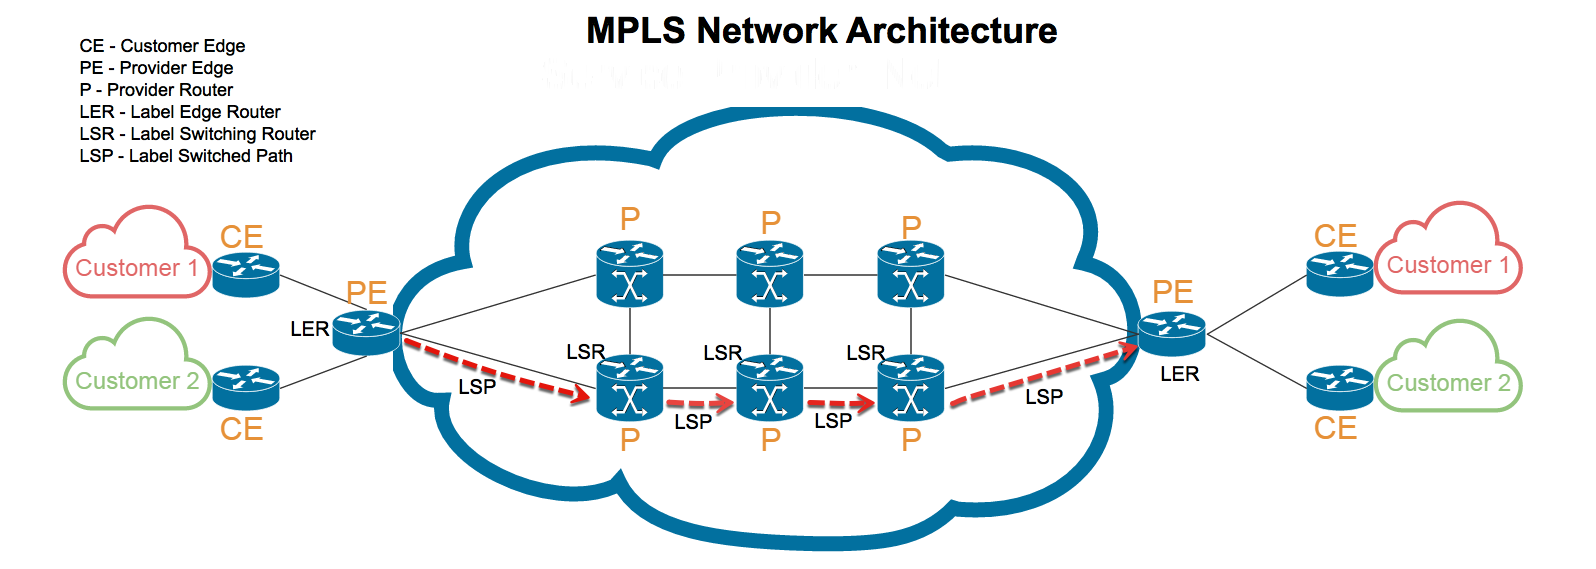
\includegraphics[scale=0.3]{Fig/RedMPLS}
    \caption{}
    \label{}
\end{figure}

\section{Características principales}
La tecnología MPLS es una solución para la conmutación multiprotocolo:

\begin{itemize}
    \item Introduce una estructura orientada a la conexión en redes que originariamente no estaban orientadas a la conexión (redes IP).
    \item Integra sin discontinuidades los niveles 2 (enlace de datos) y 3 (red) del modelo OSI, combinando las funciones de control de enrutamiento con efectividad en la conmutación.
    \item Optimiza el enrutamiento, reduciendo notablemente la complejidad de los algoritmos.
    \item Mantiene un estado de la comunicación entre dos nodos.
    \item Permite introducir QoS en redes IP.
    \item Optimiza el establecimiento de túneles en las VPN.
    
\end{itemize}

Robado de: \url{https://revistacloud.com/tecnologia-mpls-servicio-redes-privadas/}


\section{Tabla comparativa}
Robar de: \url{https://ipwithease.com/mpls-vs-ip-routing/}

\section{Fuentes}
\begin{enumerate}
    \item Principal: \url{https://www.ramonmillan.com/tutoriales/mpls.php}
    \item Sobre FEC: \url{https://www.networkworld.com/article/2350449/understanding-the-role-of-fecs-in-mpls.html}
\end{enumerate}




\end{document}